\documentclass[a4paper]{article}
\usepackage[skip=13pt]{parskip}
\usepackage{bm} 
\usepackage{graphicx} 
\usepackage{amsmath} 
\usepackage{amsfonts}
\usepackage{wrapfig} 
\usepackage{setspace} 
\usepackage{lipsum} 
\usepackage{cite}
\usepackage{csquotes} 

\setstretch{1.25}
\setlength\parindent{0pt}

\title {\textbf{An Analysis of Chronometric Cosmology and The CMB}}
\author{Nathan Burwig}
\date  {\today}

\begin{document}
    \maketitle

    \begin{abstract}
        The Cosmic Microwave Background Radiation is often taken as a
        cornerstone of evidence in contribution to the Standard Model of
        Cosmology. In the standard model, the CMB is taken to be the light last
        scattered from the hot and dense plasma permeating the early universe
        as it cooled approximately 300,000 years after the Big Bang. In this
        paper, however, the CMB is analyzed from an alternative cosmological
        model known as The Chronometric Cosmological model. This model
        considers the spatial component of the cosmos to be a 3-sphere in which
        light is permitted to take several circuits around the universe before
        potentially scattering. It is through the phenomenon of light taking
        circuits about the universe that one can derive the same notion of the
        CMB in this model. Thus, this paper endeavors to utilize this
        theoretical framework to derive first order approximations of the
        average temperature of the CMB as well as its power spectrum in this
        model and determine whether or not the model is falsified in light of
        modern astrophysical data.
    \end{abstract}

    \newpage
    \tableofcontents
    \newpage

    \section{\textbf{Introduction}}
    In 1927, Georges Lema\^{i}tre presented a paper proposing a solution to
    Einstein's field equations in which the universe was expanding.
    %In 1927 a paper was published by a man in Belgium in which a compelling
    %solution to Einstein's field equations were made. The man behind the paper,
    %Georges Lema\^{i}tre, had discovered a solution in which the universe was
    %expanding. 
    Unbeknownst to Lema\^{i}tre, however, this solution had already
    been derived several years prior by Alexander Friedmann, but notably,
    Friedmann did not place much weight on his derivation. During the early
    1920s, Friedmann produced many solutions to Einstein's field
    equations, and was largely concerned with the range of possible solutions
    as opposed to which of them could be considered the most physical.
    Lema\^{i}tre, however, attacked the problem of the expanding cosmos in
    order to attempt to understand how an expanding universe would impact
    physical theories. 
    %%
    %% The following was originally a different paragraph but it seems i maybe
    %%got some of the history wrong so I will shorten it for now.
    %%
    %Lema\^{i}tre's dedication to pursuing the possibility of an expanding
    %universe led him to a rather unique prediction. He supposed that if the
    %universe were expanding, the galaxies and other bodies in the cosmos would
    %be percieved as \textit{redshifted} due to their outward radial velocity.
    %With this he predicted of Hubbles constant and an
    %early iteration of what would become Hubble's law \cite{phyouni}. In a
    %single paper, Georges Lema\^{i}tre had laid the foundation for what would
    %become one of the most robust theories in all of modern physics; The Big
    %Bang Cosmological Model, or what is, today, commonly referred to as the
    %Standard Cosmological Model (SCM). 
    Over the course of a century the Standard Cosmological Model (SCM) would
    change form slightly, adapting to more and more astrophysical data, however
    it still remains a titan in the field of cosmology whose predictive
    capabilities have no true rival.
    
    %Astrophysics as a field is facing one of the most exciting times in history
    %where the development of increasingly sophisticated technology has ushered
    %in measurements with accuracy previously unknown to humankind. In
    %particular, the launch and initialization of the James Web Space Telescope
    %(JWST) in December 2021 and throughout early 2022 has been a revolutionary
    %moment in modern astrophysics. Since then, JWST has provided physicists of
    %various fields countless opportunities to verify or otherwise test the
    %validity of modern cosmology to an even higher degree of accuracy than the
    %previous generation of orbital telescopes has allowed. Among these theories
    %we find the Standard Cosmological Model (SCM) (also called $\Lambda CDM$ or
    %the Big Bang Theory); a true giant in the field of cosmology.
    

    %\begin{center}
    %    [This whole section needs reworking because the transition here doesn't
    %    make sense,,, need to add a section here to tie it together more]
    %\end{center}

    The SCM posits that the universe was once an incredibly dense sea of
    energy, too dense in fact for the formation of familiar matter to take
    place. This dense sea of energy eventually underwent a period of rapid
    inflation thus beginning the universe as we know it. The exponentially
    expanding cosmic soup of energy would eventually slow its rate of
    inflation allowing the matter within it to cool substantially causing more
    familiar states of matter to form. Over the span of billions of years, this
    matter would become stars, galaxies, quasars, and all the other
    wonderful celestial bodies humanity has been familiarizing ourselves with
    over the last several millennium.

    This theory would gain much traction after certain astrophysical phenomena
    were discovered. The redshift was the first of these phenomena,
    and it was its detection that set the SCM in motion, setting a precedent
    for field equation solutions which involved an expanding universe.

    In the Big Bang model,
    the cosmological redshift is attributed to the expansion of the universe
    and is generally a product of the light travelling through a space as the
    space expands. Heuristically this can be thought of as though the
    wavelength of the light is being stretched as the space it is traversing
    expands with it. It would be Hubble in 1929 who first characterized
    the redshift relation, as he noticed distant galaxies appeared to be more
    redshifted than those nearer. This solidified Hubble's Law in the history
    of physics, which is a linear redshift relation given by 
    %%
    %% Commenting out because it doesn't fit with the previous edit
    %%
    %Along with the large structure formation of the universe, the SCM notably
    %can predict two of the largest cosmological phenomena. The first being the
    %previously alluded to cosmological redshift. The cosmological redshift in
    %the SCM is considered to be a byproduct of the expanding cosmos where the
    %spectra of light is redshifted as the light travels through the expanding
    %universe. Heuristically it is often described as though the wavelength of
    %the light is being stretched as the space it travels through expands. This
    %redshift has a distinct pattern, and in 1929 Hubble would define it
    %characteristically through Hubble's Law, solidifying the redshift relation
    %in the SCM as a linear relationship given by
    \begin{equation}
        v = H_0D
    \end{equation}
    for $D$ the proper distance, $v$ the recessional velocity, and $H_0$ the
    Hubble parameter. 

    The second phenomena that has served a critical role in the formulation of
    the SCM is the Cosmic Microwave Background (CMB). The CMB in a completely
    phenomenological context is a faint glow of microwave frequency light
    permeating the universe. It has a spectrum which is very nearly a black
    body spectrum of temperature $\sim 2.7$ K. However, the CMB exhibits
    fluctuations in temperature (fractional deviations from the average $\Delta
    T/\langle T \rangle$) on the order of $10^{-5}$.
    \cite{cmb4ped}.

    In the SCM, the CMB is explained in the context of the Big Bang and the
    years nearly following the first moments of the universe. Principally it is
    considered to be the last scattering of light in the early universe as the
    hot ionized matter in the universe gradually cooled. Eventually, it would
    cool enough to deionize allowing it to become transparent to radiation.
    Thus light would scatter freely to form the CMB which we see in microwave
    telescopes today \cite{cmb4ped}. 

    The CMB, along with the cosmological redshift, make up two of the most
    physically important phenomena in modern cosmology, and the derivation and
    explanation of them is critical for any theory which wishes to exert
    explanatory power in the field. Few theoretical frameworks exist which can
    aptly do so, however few is far from none, and if a potential model proposes an
    explanation of the universe which is able to reproduce these crucial
    phenomena, it is certainly worthy of earnest investigation.

    
    \subsection{Organization of this thesis}
    This thesis centers around one such alternate cosmological model and in
    particular its ability to offer a sufficient explanation for the
    CMB in a universe far outside the current mainstream of
    modern cosmology. The model itself is known as the Chronometric
    Cosmological Model (CCM) \cite{segal} and is class of models with positive
    (spherical) curvature. Further, it is a completely static model and thus
    has no conception of the expansion or contraction of the universe or any
    notion of a beginning to the universe. It is considered infinite
    temporally.

    This thesis will first discuss the Big Bang model and some of its
    pertinent mathematical properties, then move into the Chronometric Model.
    The Chronometric Model's mathematical properties will be discussed without
    explicitly deriving them (an exercise best left to someone of a more purely
    mathematical inclination). The discussion will then turn to deriving
    certain important equations in dealing this this universe, namely the
    "Area" and "Volume" of the cosmos in this model, and a method of acquiring
    averages over this universe. It will then be possible, using averaging
    techniques, to make certain determinations about the CMB in the CCM, which
    will be discussed in section 3.

    Section 4 will then concern itself with the power spectrum of the CMB and
    how possible calculations of this spectrum are impacted based on various
    parameters. Finally, we will conclude with a general discussion of the
    limits and implications of the contents of this thesis in the scope of
    modern cosmology, along with further points of research to be explored.

    A pertinent question might be related to why this thesis will not be
    discussing aspects of the cosmological redshift. The reason for this is due
    to a preexisting (and rather complete) discussion of the redshift having
    already been conducted by a research colleague Maxwell Kaye in \cite{kaye}
    and, of course, in Segal \cite{segal_b}

    \newpage

    \section{\textbf{The Models}}
    In science, theories are formulated to explain phenomena and are constantly
    tested through empirical observation and experimentation. Robust theories
    that can successfully explain and predict the observed phenomena are
    generally not subject to modification or reformulation, while theories that
    fail to do so are subject to revision or replacement. Thus, a natural
    question when discussing alternate cosmological models is:
    \textit{is there anything wrong with the current model}?

    The answer is to this question is not particularly straightforward. As
    stated previously, the SCM has proven to be a reliable and robust framework
    for understanding the universe. It has successfully predicted and explained
    a wide spread of phenomena. This is not to say, however, that the model
    does not have any unresolved issues. Over the course of the last century,
    many such issues have been resolved, but as telescopes continue probing
    deeper and deeper into universe with progressively more advanced means of
    measurement, they may yet find more unsolved mysteries.

    One such example which has become pertinent quite recently is related to
    large structure formation in the early universe. In a paper by Labb\'{e} et
    al., the James Webb Space Telescope (JWST) was utilized to observe galaxies
    at large redshift ($z=7.4$ to $z=9.1$). In their paper, they found that
    these galaxies were of uncharacteristically large masses given their age.
    One such galaxy was discovered to have a redshift of 7.5 while having a
    higher fiducial mass than that of the Milky Way\cite{labbe}. In their paper titled \textit{A population of red candidate massive galaxies $\sim$600 Myr after
    the Big Bang} by Labb\`{e} et al. reported the following.

    \begin{displayquote}
        Galaxies with stellar masses as high as $\sim 10^{11}$ solar masses
        have been identified out to redshifts z $\sim$ 6, approximately one
        billion years after the Big Bang... Here we make use of the 1-5 $\mu$m
        coverage of the JWST early release observations to search for 
        intrinsically red galaxies in the first $\approx$ 750 million years of cosmic
        history. In the survey area, we find six candidate massive galaxies
        (stellar mass $> 10^{10}$ solar masses) at $7.4 \le z \le 9.1$, 500–700 Myr
        after the Big Bang, including one galaxy with a possible stellar mass
        of $\sim 10^{11}$  solar masses. If verified with spectroscopy, the stellar
        mass density in massive  galaxies would be much higher than
        anticipated from previous studies based on rest frame
        ultraviolet-selected samples.
    \end{displayquote}

    In all, the paper goes on to describe possible explanations for such a
    discrepancy at such a large redshift, but in general we can see this as a
    clear example of how possible mysteries can arise in modern cosmology
    \cite{labbe}.

    Another example of unresolved issues in the SCM can be found in the
    cosmological redshift. For much of the model's existence, the cosmological
    redshift has existed as means by which light seemingly loses energy by no
    apparent mechanism. The wavelength of the light is simply "stretched"
    causing its energy to vanish into the cosmos. This problem would
    eventually be dubbed the \textit{cosmic sink} by Hermann Bondi, and it is a
    problem which led to dissatisfaction amongst some physicists. This
    eventually became the starting point for Irving Segal who was troubled by
    this apparent violation of the conservation of energy. In hopes of
    restoring this grand scale energy conservation, Segal developed the
    Chronometric Cosmology\footnotemark.

    Segal had considered closely the work of Oswald Veblen on group
    deformations and particle classification of conformal space, and used these
    ideas formulated to begin considerations of a conformal
    spacetime \cite{segal_b}. These considerations were motivated in part by
    the formulation of quantum mechanics and special relativity. Special
    relativity displaced Galilean relativity which in turn became a sort of
    limiting case of special relativity. In the same way, classical mechanics had
    started to be considered as a limiting case of a more fundamental theory --
    quantum mechanics. Perhaps, then, the ideas put forth by Minkowski could
    be considered a limiting case of a larger, more accurate formulation of
    cosmology.

    \footnotetext{This development was primarily conducted via his 1976 book
    \textit{Mathematical Cosmology and Extragalactic Astronomy}\cite{segal_b},
    however much of the mathematical framework regarding the CMB is found in other
    papers such as \cite{segal_cmb} and \cite{segal_spinor}}

    \subsection{Development of the Chronometric Cosmos}
    Segal's development of the chronometric cosmology starts with an axiomatic
    framework through which one can develop any generalized cosmos. The axioms
    given in \cite{segal_b} are as follows.

    \begin{enumerate}
        \item The Cosmos is a four-dimensional manifold\footnotemark.
        \item At each point in the cosmos there exists and infinitesimal 
            notion of causality.
        \item The cosmos is globally causal in the sense that it admits no 
            closed timelike loops.
        \item The cosmos can be locally separated into spatial and temporal components
    \end{enumerate}

    \footnotetext{One must go out of their way to note the exclusion of the
    singularity from this definition, however the general principle applied is
    that if you were to remove singularities from consideration you would be left
    with a four-dimensional manifold from which you could then consider the
    adjunction of singularities \cite{segal_b}.}

    While the exact nature of these axioms is outside the scope of this
    thesis\footnotemark, they outline the mathematical properties of the
    framework utilized by Segal, and they are based on common notions and
    intuitions about the universe in general \cite{segal_b}. In the context of
    this paper, a few of the axioms stand out in particular. 

    Axiom 2 indicates that at each point in the four-dimensional manifold,
    there exists a notion of causality. Formally, this means that at every
    point in space there is a nontrivial closed convex cone tangent to that
    point in space. This is considered to be the functional description of a
    light cone in the axiomatic description set forth by Segal. Further, axiom
    3 admits stationary observers which also implies the cosmos has a global
    notion of causality and that there can be no close time-like paths (hence
    $\mathbb{R} \times \mathbb{S}^3$, $\mathbb{R}$ being the temporal
    component) \cite{segal_b}. These axioms, then, clearly derive notions which
    are already quite familiar to the field of cosmology, just in a more
    general way.

    In the same way, the cosmos being a four-dimensional manifold is certainly
    not a new concept, but it, along with the other axioms, limits the space of
    possible world manifolds by a considerable degree. In fact, Segal shows
    that, given the axioms above, there are only two admissible world
    manifolds\cite{segal_b}. 

    \footnotetext{Again a more complete analysis is found in \cite{segal_b} and
    \cite{kaye}}

    \subsubsection{Admissible Manifolds}
    Throughout the course of \cite{segal_b}, Segal shows that the only two
    admissible world manifolds are:
    \[
        M = \mathbb{R} \times \mathbb{R}^3 \;\;\;\;\;\; 
        \bar{M} = \mathbb{R} \times \mathbb{S}^3
    \]
    Where here we refer to $M$ as the standard Minkowski space and $\bar{M}$ as
    the universal cosmos. $M$ is then taken to be isomorphic to $\mathbb{R}^4$
    and $\bar{M}$ is isomorphic to $\mathbb{R} \times \mathbb{S}^3$. While
    these distinctions become important for large scale astrophysical
    phenomenon, Segal found that for smaller scale interactions  $\bar{M}$ is
    functionally indistinguishable from $M$. This is essentially the same
    effect as a tangent plane on the surface of a sphere being nearly identical
    with the surface of the sphere in a local approximation. 

    \subsubsection{The Metric}
    Briefly, now, we return to the work of Lema\^{i}tre and Friedmann. They
    initially (separately) derived the expanding solution of Einstein's field
    equations in the 1920s, and later this work would be picked up by Robertson
    and Walker. This would then become the Friedmann-Lema\^{i}tre-Robertson-Walker
    metric which would go on to be a critical component for understanding the
    general characteristics of any cosmological model.

    In general, a metric determines the distance between any two points in a
    space. It is essentially a distance function in its most basic form, and
    the FLRW metric, in its most general form, is as follows
    \begin{equation}
        dl^2 = R(t)^2\left(\frac{dr^2}{1-kr^2} + r^2 (d\theta^2 +
            \sin^2(\theta)d\phi^2)\right)    
    \end{equation}
    Where $R$ is a scaling factor which in general for the SCM is taken to be
    a function of time to account for the expansion of the universe. The
    parameter $k$ is constant which characterizes the curvature of the space
    which the metric describes. It can take on three possible values:
    \begin{itemize}
        \item $k=+1 \;\;\rightarrow$ closed/spherical space.
        \item $k=0 \;\;\;\;\;\rightarrow$ euclidean/flat space.
        \item $k=-1 \;\;\rightarrow$ open/hyperbolic space.
    \end{itemize}
    Thus the standard Minkowski spacetime $M$ has the constant $k$ set to zero,
    converting equation (2) into the following.
    \begin{equation}
        dl^2 = R^2\left(dr^2 + r^2d\theta^2 + r^2 \sin^2(\theta) d\phi^2\right)    
    \end{equation}
    This can be identified with the general volume component in spherical
    coordinates of typical Euclidean space (merely scaled by the $R$ factor. In
    fact, if we take the more general form of the metric, the metric tensor,
    and we utilize the property of the metric tensor which relates the square
    root of the determinant of the metric tensor to the volume component in the
    space described by the metric, we will see exactly how they relate.

    The FLRW metric tensor is given as
    follows.
    \[
        g = 
        R^2
        \begin{pmatrix}
            \frac{1}{1-kr^2}  & 0 & 0 \\
            0 & r^2 & 0 \\
            0 & 0 & r^2\sin^2(\theta)
        \end{pmatrix}
    \]
    And the general volume is then...
    \[
        V(r) = \int{ \sqrt{det(g)}\; d\Omega}
    \]
    Which for Minkwoski space ($k = 0$, given that $d\Omega$ in this context is
    the spherical coordinate measure $dr d\theta d\phi$) becomes
    \[
        V(r) = R^2 \int_0^{r} r^2\;dr 
                   \int_0^{2} \sin(\theta)\;d\theta
                   \int_0^{2\pi}\;d\phi
    \]
    Where we are integrating for some volume enclosed by $Rr$ at some arbitrary
    time $t_0$ so we will take $R=R_0$ at $t_0$ resulting in the following.
    \begin{equation}
        V(r) = \frac{4}{3} \pi (R_0 r)^3
    \end{equation}
    Which is in fact exactly what we would expect for the volume enclosed by
    some region of $M$. We can conduct an identical calculation to determine
    what this volume will be for $\bar{M}$.
    \begin{align*}
        V(r) &= R^2 \int_0^{Rr} \frac{r^2}{\sqrt{1-r^2}} \;dr 
                   \int_0^{\pi/2} \sin(\theta)\;d\theta
                   \int_0^{2\pi}\;d\phi         \\
             &= 2 \pi R^3 \left[\;\sin^{-1}(r) - r\sqrt{1 - r^2}\;\right]
    \end{align*}
    This however is a rather awkward form for a handful of reasons. One is that
    it is offering the volume enclosed by a certain region of $\bar{M}$ in
    terms of the total radius of the space ($\mathbb{S}^3$) and the
    \textit{coordinate} $r$. The coordinate $r$ in this case is not a
    particularly physical concept as it describes a \textit{local} distance as
    opposed to the \textit{manifold} distance. Pulling a lower dimensional
    example, we take an ant living on the two dimensional surface of
    $\mathbb{S}^2$. The coordinate $r$ then would be akin to taking the taking
    the tangent plane at the current position of the ant and moving it from
    $\mathbb{S}^2$ onto that tangent plane, then letting it walk across that
    surface. It would eventually be walking some distance "above" the surface
    of its original space. As put by Max Kaye in \cite{kaye} "...imagine a
    sheet of glass balanced perfectly on the north pole of a sphere. The
    distance from the north pole to any other point p on the sphere, measured
    by r, would be the distance along the sheet of glass an ant must walk such
    that it is standing directly above the point p"

    \footnotetext{Explicitly we should be calling this the hypersurface and
        consequently the hypersurface area and hypervolume. However, for the
        sake of readability and writing slightly more succinctly, we will
        generally refer to the hypersurface area/hypersurface and hypervolume
        as surface area/surface and volume respectively}

    Another reason for which one may find this expression awkward is the
    arcsin which, granted, is an argument of beauty, however it is not without
    validity. The universe being described by these equations is highly
    unfamiliar, thus we desire to put it in a more appreciable form such that
    an intuition about the space can be formed.

    The simplification we desire is found by utilizing the manifold distance as
    opposed to $r$. We know that the relationship between the metric distance
    $l$ and the coordinate $r$ comes from general radial paths. This means we
    take $d\theta = d\phi = 0$ in (2) for $k = 1$ which gives us the following.
    \begin{equation}
        l = R\int_0^r \frac{dr}{\sqrt{1-r^2}}\; dr = R\sin^{-1}(r) 
    \end{equation}
    Thus
    \begin{equation}
        r = \sin(\frac{l}{R}) = \sin(\rho)
    \end{equation}
    Here the quantity $l/R$ is a dimensionless quantity which is typically how
    distance is described in $\bar{M}$ and is exactly the manifold distance
    mentioned above. We now give the distance between objects on the surface of
    this universe, not as an ant on a sheet of glass, but as an ant crawling
    across the surface, which is a far more natural and physical coordinate.

    Here it is also worth noting that, while in general $R$ is a scaling factor
    and may depend on time, in the CCM $R$ is taken to be static and exactly
    the radius of the universe.

    Substituting equation (6) back into the general volume expression, and
    calling $l/R$ as $\rho$, results in the following equation.
    \begin{equation}
        V(\rho) = 2 \pi R^3 \left[ \rho - \cos(\rho)\sin(\rho) \right]
    \end{equation}
    Where $\rho \in (0,\pi)$. 

    Interestingly, if we expand this equation out in terms of small $\rho$, we see
    the following.
    \begin{equation*}
        V(\rho) \approx \frac{4\pi}{3} R^3 \rho^3 \left[1 - \frac{\rho^2}{5} +
        \cdots \right] 
    \end{equation*}
    Which shows us that $\rho$ must be close to 1 in order for deviations from
    the geometry of $M$ can be noticed.

    A unique result of having an expression such as this, is that it allows us
    to make averages over the whole of $\bar{M}$ as one typically would in
    $M$. This can be done by the useful relationship between the surface area
    of n-spheres and their volumes, which dictates that the surface area is
    exactly the derivative of the volume. Using this will allow us to a) easily
    derive the following expression for the surface area of $\mathbb{S}^3$ and
    b) normalize the surface area (again surface area being the actual volume
    of $\bar{M}$ which forms spacetime in the CCM) to allow for easy averaging
    over functions of $\rho$. $A(\rho)$ is then...
    \begin{equation}
        A(\rho) = 4 \pi R^2 \sin^2(\rho)
    \end{equation}
    The discussion of how to utilize these two expressions to take averages
    over the cosmos will be discussed and further utilized in section 3.1.3

    %basically want to start with the axioms then move into there being only two
    %admissable world manifolds. be sure to mention that M is embedded in barM,
    %and to mention the motivation being from conformally symmetric groups

    %The Chronometric Cosmological Model is one that describes a universe
    %vastly different in character than that which most are used to. As such it
    %is worth devoting a portion of this writing to a qualitative description of
    %this universe, and how one can explain the cornerstones of any good
    %cosmological model (redshift and CMB) within the CCM. 

    %That said, in order to aptly describe the CCM, we should first recap
    %and familiarize ourselves with the relevant physical and mathematical properties 
    %in SCM.



    %\subsection{The Standard Picture}
    %There are several unique properties of the 
    %\subsection{Motivation}
    %\subsection{The Metric}
    %\subsection{The Cosmological Redshift}
    %\subsection{The Chronometric Cosmology}
    %swith cosmic sink
    %\subsubsection{Development}

    \newpage

    \section{\textbf{The Cosmic Microwave Background}}
    %The explanation of the CMB from the perspective of the SCM has already been
    %discusses, however it has not been sufficiently explained within the
    %framework of the CCM.
    \subsection{Average Temperature of CMB}
    
    The average temperature of the CMB is a critical aspect of the CMB as a
    phenomenon in the universe. This, along with the power spectrum characterize
    the primary features of the CMB, and thus, if the chronometric model is able to
    reproduce these aspects of the CMB, we can say that the model is, if nothing
    else, not falsified in light of modern astrophysical data. In order to
    determine these attributes from first principle, however, it is important to
    first get the bigger picture of how the CMB is accounted for within this model.
    
    Light in the chronometric cosmos is broadly separated into two categories. The
    first we call pristine light, and the second we call residual. We call the
    light that has taken fewer than one half-cycle about the cosmos pristine and
    the light which has passed the $\rho = \pi$ manifold distance residual. The CMB
    then is concerned primarily with the residual light in the universe. 
    
    Given the relative sparsity of matter in the universe, light of this category
    would be able to take many circuits about the universe. The infinite time for
    this high-dispersion radiation to accumulate would directly imply that it is
    qualitatively distributed in accordance to Planck’s law, and thus is in fact a
    black body spectrum. This fact is shown more formally in \cite{segal_cmb},
    but here will be taken as a fact.
    
    It is worth noting before continuing that the origin of this light is
    unimportant for general considerations.  However for a more specific analysis
    we can easily consider the source of the pristine and residual  light in the
    universe to be the galaxies and other luminous matter in the universe. 

    %To show that the residual light is characteristic of a black body spectrum, we
    %need only point to the stochastic nature of of the emission and motion of
    %galaxies and other luminous material.


    \subsubsection{Methodology}
    
    The  methodology, then, for determining the average temperature of the CMB
    in this model will be to utilize the residual light in the cosmos. The
    residual light will be considered explicitly as the light "left over" after
    traversing multiple half circuits of the cosmos, and is thus the
    light which has \textit{not} gone extinct. The residual light is considered
    to be of particular importance as, given the curvature of $\bar{M}$, it is
    allowed to continue traversing the universe becoming of higher and higher
    dispersion, directly contributing to the CMB.

    This analysis will be quite general and is only intended to act as a first
    order approximation to the average temperature to the CMB. As such, a
    handful of approximations must be clarified. We will consider
    all galaxies to be \textit{approximately} the same in radius ($d$),
    luminosity ($L$), and have an explicit number count ($N$). Each galaxy is
    approximated as a perfect absorbing sphere as well as an emitter of light.
    Using these factors we will calculate on average the amounts of pristine
    and residual light in the universe, and what of that reaches the Earth
    which will give us qualitative information regarding the CMB in this model.
    We will then utilize that to determine a range of values for the average
    temperature of the CMB.

    \subsubsection{Extinction Law}
    For a general order of magnitude estimate of the total radiative flux of
    the CMB which arrives at the Earth in the $\mathbb{S}^3$ cosmos, we first
    need to consider extinction of light as light takes half-circuits about
    the closed universe. 

    In general, we know that that the rate of change of photons ($N_p$)
    traversing $\bar{M}$ will be negative and proportional to the number of
    half-circuits ($n$) in accordance with general stochastic
    absorption of light. Using this simple relationship we can construct the
    following.
    \begin{equation*}
        \frac{dN_p}{dn} = -\alpha n \; \longrightarrow\; N_p=N_{p_0}e^{-\alpha n}
    \end{equation*}
    For $N_{p_0}$ the amount of light which has not yet taken a half circuit
    about the universe at some arbitrary time $t_0$, which formally makes it the
    pristine light $P$. This allows us to consider the total amount of
    residual light $N_{p_0}$.
    \begin{equation*}
        N_{p} = N_{p_0}e^{-\alpha n} 
    \end{equation*}
    With the identification of $N_{p_0}$ as the pristine light $P$, we can then
    arrive at the following expression for the residual light in the universe.
    \begin{equation}
        N_p=Pe^{-\alpha n}
    \end{equation}
    This expression is of course per half-circuit $n$. For the purposes of
    determining the extinction of light over any $n$ circuits the summation
    to infinity must be taken. For the purposes of this analysis, $n$ will be
    taken to start at 1 as this must be an examination of the residual light
    implying at least one half-circuit has been taken.
    \begin{equation*}
        P\; \sum_{n=1}^{\infty} e^{-\alpha n} = P \left[e^{-\alpha} +
            e^{-2\alpha} + \cdots \right] = \frac{P}{1-e^{-\alpha}} 
    \end{equation*}
    In order to further simplify this expression an approximation
    via Taylor Series expansion is utilized. Given the Taylor series expansion
    for $e^{-\alpha}$, the following is known.
    \begin{equation*}
        e^{-\alpha} = 1 - \alpha + O[\alpha]^2
    \end{equation*}
    From here all greater order terms will be taken as negligible as, for
    general considerations $\alpha$ is considerably less than one\footnotemark
    \cite{segal_b}. Removing the higher order terms in this approximation
    allows for a massive simplification in the given expression leaving us with
    the following.
    \begin{equation}
        N_p \approx P\alpha^{-1}
    \end{equation}
    Before continuing on to determine what exactly these parameters are in the
    context of the CCM, we should stop briefly to consider the physical meaning
    of this expression.
    
    \footnotetext{This will be shown more clearly in 3.1.3}

    In typical considerations of the standard flat Minkowski spacetime $M$, as
    light radiates away from emitters, it is free to traverse the infinite
    plane of the cosmos until it is scattered. Thus, the average amount of
    light will always decrease irrespective of continuous emission of light
    from other sources in the cosmos. However, in the case of $\bar{M}$, light
    is permitted to continue taking circuits about the universe while the
    emitters continue radiating. Because $P$ is constant the residual light
    will contribute to the net luminous flux over many cycles as an enhancement
    factor of sorts. This is precisely what allows the CMB to take form in the
    CCM. In this way, we can consider that from the theoretical framework of
    Segal's model, the CMB is not merely retrofitted, but it is, in fact,
    \textit{predicted}.

    The next steps, then, are of course to consider how we can determine the
    approximate values for the pristine light and the absorption coefficient
    $\alpha$ from the principles already discussed in the CCM.

    \subsubsection{Absorption Factor}

    To start, we consider how one can calculate the absorption factor as it
    relates to the residual light in the cosmos. As stated before, we consider
    this light to be the light which has \textit{not} gone extinct. In this
    case, then, we need only consider the amount of light that arrives at the
    Earth, as this is the only light which we can factor into the chronometric
    model's explanation of the CMB. In order to calculate this, then, we can
    shift the question to be how much light is absorbed by galaxies in the
    universe en route to the Earth?

    We consider the general volume of $\mathbb{S}^3$  as a
    function of the manifold distance $\rho$.

    \begin{equation*}
        V(\rho) = 2 \pi R^3 \left[\rho-\cos(\rho)\sin(\rho)\right]
    \end{equation*}

    %\footnotetext{It is worth noting that in Segal's own work he develops a
    %slightly different equation for the volume of $\mathbb{S}^3$. The exact
    %expression he derives, however, is only a modulus of the expression we
    %have derived in the context of this thesis, and is thus treated as only
    %varying by some constants (in this case it varies by $4 \pi R^3$). It will
    %later become apparent that these constants are of little significance to
    %the endpoint of this calculation.}

    We can then characterize the surface area as follows based on the analysis
    conducted in 2.1.2.
    \begin{equation}
        A(\rho) = 4 \pi R^2 \sin^2(\rho)
    \end{equation}
    As discussed previously, we can utilize these expressions to develop
    a general expression for the normalized surface area over $\mathbb{S}^3$.
    We derive the following normalization factor over the integral from $0$ to
    $\pi$ (ie the entire surface).
    \begin{equation}
        Q = \int^\pi_0 A(\rho) \;d\rho
          = \int^\pi_0 4 \pi R^3 \sin^2(\rho) \;d\rho
          = 2 \pi^2 R^3
    \end{equation}
    We note the change in power of $R$ from $R^2$ to $R^3$ comes from the fact
    that $\rho$ is defined in terms of R. The integral in terms of $d\rho$
    picks up a factor of $R$ due to the fact that $dl = R\;d\rho$ where the
    original integral in terms of $dl$ would go from $0$ to $\pi R$.
    
    From here we can find the average value of any function of $\rho$ by
    utilizing this normalization factor in the following way.
    \begin{equation}
        F(\rho) = \int_0^\pi \frac{A(\rho)}{Q} \; f(\rho) \;d\rho
    \end{equation}
    Where the integral goes from 0 to $\pi$ for the sake of averaging over the
    entire surface (ie cosmos).

    With this framework we can now turn our attention to what exactly it is we
    wish to be finding the average value of. It has been noted that we are
    interested in the amount of light occluded by our approximated galaxy
    objects at any given point in the cosmos (for posterity we consider Earth
    to be our point of relevance). Thus we are interested purely in the
    percentage of the sky taken up by such objects, and therefore we want to
    know the percentage of solid angle taken up by $N$ galaxies.

    We define the solid angle as the field of view obstructed by an object at
    some distance. In the consideration of celestial bodies, we can simply take
    the solid angle to be given as follows.
    \begin{equation*}
        \Omega = 2\pi\left(1-\cos(\theta)\right) = 4\pi\sin^2\left(\frac{\theta}{2}\right) 
    \end{equation*}
    We now consider that for any general consideration of a distribution of
    galaxies, we can consider them to be quite far away. Thus, utilizing small
    angle approximations, we can arrive at the following.
    \begin{equation}
        \Omega = \pi \theta^2
    \end{equation}
    Or the area of the central cross section of our sphere typically called the
    great circle of our sphere. In this approximation, $\theta$ is
    characterizing the radius of of the great circle of the sphere. Thus
    $\theta$ is formally $d$ in the small angle approximation.

    For considerations of the ratio of the sky obstructed by the absorbing
    spheres, we must carefully consider the geometry of the situation. If it
    were the case that we were in typical flat Minkowski space $M$, then we
    would take no issue and simply take our ratio with respect to the total
    surface area of the sphere which we project or solid angle onto. However,
    given that, in $\bar{M}$ an object at $\rho=\frac{\pi}{4}$ and an object at
    $\rho=\frac{3\pi}{4}$ will take up the same $\Omega$, we must utilize the
    surface area component of $\mathbb{S}^3$. Thus, our equation for the ratio
    of solid angle obstructed by a single spherical absorber of radius $d$
    becomes the following.
    \begin{equation*}
        \frac{\Omega}{\Omega_{total}} = \frac{\pi d^2}{4 \pi R^2 \sin^2(\rho)} 
    \end{equation*}
    Thus for a general case of $N$ such bodies we arrive at...
    \begin{equation*}
        \frac{\Omega}{\Omega_{total}} = \frac{N \pi d^2}{4 \pi R^2 \sin^2(\rho)} 
    \end{equation*}
    Now we can consider the average based on our formulation of equation (5)
    substituting $\frac{\Omega}{\Omega_{total}}$ for $f(\rho)$. 
    \begin{equation*}
        F_{\Omega}(\rho) = \int_0^\pi \frac{A(\rho)}{Q} 
        \;        \frac{\Omega}{\Omega_{total}}  \;d\rho 
                 = \int_0^\pi \frac{N d^2}{2 \pi R^2} \;d\rho
    \end{equation*}
    Thus...
    \begin{equation}
        F_{\Omega}(\rho)= \frac{N d^2}{2 R^2} 
    \end{equation}
    This value for the average absorption of light is in fact exactly 
    identified as the absorption factor $\alpha$ in (3). We note that it is
    obvious given the inverse cubic relationship to the radius of the
    $\mathbb{S}^3$ cosmos that $\alpha$ must be less than 1.


    \subsubsection{Pristine Light Calculation}
    The consideration of the pristine light in the cosmos will follow very
    similarly to the former as the calculation is yet another average over the
    cosmos. Now, however, it is not about their properties as absorbers, but
    instead their properties as emitters. 

    As stated, we consider each galaxy to have identical properties for the
    sake of a first (or zeroth) order calculation. As such we take each galaxy
    to have uniform luminosity $L$, and define their flux as follows.
    \begin{equation}
        \phi = \frac{L}{4\pi R^2 \sin^2(\rho)} 
    \end{equation}
    Thus, our average becomes the following.
    \begin{equation}
        F_{\phi} = \int_0^{\pi}\frac{A(\rho)}{Q} \frac{NL}{4 \pi R^2
               \sin^2(\rho)}\;d\rho = \frac{NL}{2 \pi R^2} 
    \end{equation}
    This is then our most general expression for the average pristine light in
    $\bar{M}$.
    %%
    %% This section deals with my calculation regarding the apparent luminosity
    %% It is interchangeable with the calculation that is uncommented which I
    %% have marked the beginning and end of.
    %%
    %\begin{equation}
    %    \phi = \frac{L}{4 \pi R^3 \sin^2(\rho)(1+z)} 
    %\end{equation}
    %Note, the $1+z$ term is thus making our $\phi$ the apparent bolometric flux
    %and $L$ the absolute bolometric flux. 

    %Typically, in $M$, one would take this same expression but with a $(1+z)^2$
    %term. However, for various geometric reasons explored at length in Kaye
    %\cite{kaye} and Sandage \cite{sandage_annurev}, the chronometric model only
    %has one such factor to scale with the redshift. Here the value of $z$ is
    %$z=\tan^2(\rho/2)$ as derived in Segal \cite{segal_b}

    %Utilizing the same scheme from section 3.1.4 we can setup our averaging
    %function as follows.
    %\begin{equation*}
    %    F_{\phi} = \int_0^{\pi} \frac{A(\rho)}{Q}  \frac{N L}{4 \pi R^3
    %           \sin^2(\rho)(1 + \tan^2(\rho))}\;d\rho 
    %\end{equation*}
    %Which we will find to integrate out to...
    %\begin{equation}
    %    F_{\phi} = \frac{LN}{4R^3} 
    %\end{equation}
    %This, then, is the most general expression in terms of the absolute
    %luminosity of the galaxies being observed, while still accounting for
    %redshift. If one conducted the same analysis without accounting for the
    %redshift in $\bar{M}$, then one would find their solution to be out by a
    %factor of $\frac{1}{2}$, which tells us that we lose exactly $\frac{1}{2}$
    %of the total flux to redshift alone.
    While it is rather useful to have an expression for any "typical point" in
    space, we here on Earth find ourselves in a rather peculiar situation.
    Namely, we happen to be located approximately half-way from the center of
    what seems to be a perfectly average spiral galaxy\footnotemark. Thus, one
    could easily formulate the luminosity $L$ in terms of the flux from the
    Milky Way within the solar neighborhood. Thus we can take $L$ to be exactly
    the following.
    \begin{equation}
        L = 4 \pi \phi_e (\frac{d}{2})^2
    \end{equation}
    Where $\phi_e$ is the aforementioned flux of the Milky Way received by the
    Earth. Notably we utilize the standard spherical surface area formula for
    this expression as the curvature of the universe is imperceptible on the
    scales of an individual galaxy and thus considerations of its larger
    topology are unnecessary.

    \footnotetext{This may or may not be the case exactly, and this will be
    discussed at greater length in 3.2.5}
    %%
    %% Keeping this one in case i want it later
    %%
    %Given that the Earth itself rests in the Milky Way galaxy, and ultimately
    %our interests are centered around determining values for the average
    %temperature of the CMB as detected on Earth, we can make a useful and
    %simplifying assumption. This is a) that the Milky Way is considered an
    %average galaxy in the cosmos\footnotemark and b) the Earth rests at
    %approximately the halfway point between the center of the galaxy and it's
    %furthest edge (at the radial point $\frac{d}{2}$).
    %
    %Conceding these assumptions, we can take the luminosity of an average
    %galaxy in terms of the flux originating from the Milky Way that is received
    %by the Earth. Doing so results in the following expression.
    %
    %From here we can utilize equation (7) to find the average pristine light in
    %terms of $\phi_e$ and given that we are approximately at $\frac{d}{2}$.
    %\begin{equation*}
    %    F_{\phi}(\rho) = \int_0^{\pi} \frac{A(\rho)}{Q} \; \frac{L}{4 \pi R^3
    %    \sin(\rho)}  \; d\rho
    %    = \int_0^{\pi} \frac{A(\rho)}{Q} \; \frac{\pi \phi_e d^2}{4 \pi R^3
    %    \sin(\rho)}  \; d\rho
    %\end{equation*}
    If we substitute (19) into (18), it results in the following.
    \begin{equation}
        F_{\phi}(\rho) = \phi_e \frac{N d^2}{2 R^2} 
    \end{equation}
    This, then, is the average pristine light $P$ in the cosmos as identified
    in (10).

    \subsubsection{Average Temperature of CMB}
    The tools for calculating the average temperature of the CMB have now been
    derived. The discussion of the average pristine and residual light in the
    cosmos has been conducted and the relationship between the two has given us
    an explicit way to calculate the total flux of light in the cosmos. Given
    expression (3), we can now substitute the calculated values of $P$ and
    $\alpha$ to see that the net flux of the CMB arriving at the Earth is
    simply $\phi_e$.
    \begin{equation}
        P\alpha^{-1} = \phi_e \frac{N d^2}{2R^2} \left[\frac{N d^2}{2
        R^2}\right]^{-1} = \phi_e
    \end{equation}
    The uniqueness of this result cannot be overstated. Due to the form of the
    calculations conducted we see that the terms relating to the radius of the
    $\mathbb{S}^3$ manifold, the number count of galaxies, and the radius of
    the average galaxy, all drop out of our expression and leave us with
    $\phi_e$. Of course, this varies under considerations of our assumptions.
    For instance, our position in the Milky Way could be closer to
    $\frac{3}{4}d$ which would alter our solution accordingly. For the purposes
    of a zeroth order calculation, however, we will consider $\frac{d}{2}$ to
    suffice.

    One factor which must be considered, however, is how the redshift will
    change this expression. Certainly, given that the pristine light will be
    coming in from some distance, the redshift must be considered. To do this
    we can find the redshift average over space given that the character of 
    the redshift factor in $\bar{M}$ is $(1+z)^{-1}$ and $z=\tan^2(\rho/ 2)
    $\cite{segal_b}.
    \begin{equation}
        F_z(\rho)=\int_0^{\pi} \frac{A(\rho)}{Q} 
                \left(1+\tan^2\left(\frac{\rho}{2}\right)\right)^{-1}
               \;d\rho = \frac{1}{2} 
    \end{equation}
    Thus, the total flux is reduced by a factor of 2 due to the redshift in
    $\bar{M}$ resulting in (21) becoming $P\alpha^{-1}=\phi_e/2$.

    The CMB in the CCM is taken to be a perfect black
    body spectrum. As such, we can utilize the Stefan-Boltzmann equation to
    determine the temperature of the radiative flux density of a black body
    spectrum.
    \begin{equation}
        J = \sigma T^4 \longrightarrow
        {T=\left[\frac{\phi_e}{2\sigma}\right]^{\frac{1}{4}}}
    \end{equation}
    For $J$, the radiative flux density which here we take to be $\phi_e$, 
    $\sigma$ the Stefan-Boltzmann constant ($5.67 × 10^{-8} \frac{W}{m^2
    K^4}$), and $T$ the temperature\footnotemark. 

    \footnotetext{It should be noted that the more general expression of the
        Stefan-Boltzmann relation includes the factor of $\epsilon$ or
        emissivity. However, the emissivity of a perfect black body is simply 1.}

    \subsubsection{Analysis of Average Temperature}
    Given the unique relationships derived above, it is now the hope to put
    them to the test of actual astrophysical data. 

    Equations (20) and (21) together show that the expected average temperature
    of the CMB power spectrum in $\bar{M}$ is given by $T =
    \left[\phi_e/2\sigma\right]^{1/4}$. In order, then, to calculate the value
    of the temperature, data regarding the flux from the Milky Way in the solar
    neighborhood is needed. 

    Several probes have made attempts at calculating this value, and to varying
    degrees of accuracy and through various methods. In \textit{The surface
    brightness of the Galaxy at the solar neighbourhood} by Melchior et al.,
    several estimates from various data sets and papers were summarized in
    discussed, along with a new synthetic estimation method proposed by the
    authors \cite{melchior}. However, the discussion of the flux is broken down
    into various frequency bands which are not able to be simply summed over.
    There is often considerable overlap between frequency bands, and
    determination of where these overlaps are and how much overlap exactly
    exists is a task which requires more precision than is perhaps required for
    such an approximate calculation. The frequency bands also do not cover the
    entire spectrum of light being emitted in most cases, thus it may not offer
    the most complete perspective. Because of these reasons, it will be
    convenient to consider this calculation from the perspective of the
    absolute luminosity $L$.

    Given equation (18), for any general emitting body (which we are
    sufficiently nearby to such that the curvature of $\bar{M}$ does not affect
    the geometry of the situation) we know the following.
    \begin{equation*}
        \phi = \frac{L}{4 \pi d^2} 
    \end{equation*}
    Thus we can simply calculate the flux of the Milky Way based on the
    luminosity of the Milky Way. This measurement is slightly more easily
    attained, and is more commonly considered in standard astrophysics, meaning
    there already exists a range of approximate values. Utilizing the
    luminosity relationship in this way also means that we must have some idea
    of how far the solar neighborhood is from the center of the galaxy.
    Typically this is taken to be the distance from Sgr A*, and it typically
    taken to be $\sim 8.3$ kpc, or $\sim 27,000$ light years
    \cite{stellar_orbits}\cite{nasa}. For the sake of attaining the correct
    units for the Stefan-Boltzmann constant ($W/m^2$), this will be converted
    into a rather large quantity of meters; $\sim 2.6 \times 10^{20}$m. 

    The luminosity itself is a rather variable parameter, and is quite tricky
    to determine for the Milky Way due to obstructions such as dust and the
    general disc of the galaxy. However, the luminosity is typically considered
    to be on the order of $\sim 1.1 \times 10^{10}$ $L_{\odot}$, or $\sim 4.2 
    \times 10^{36}$ Watts\cite{local_group}.

    For these given values of $L$ and $d$, utilizing equations (20) and (21)
    result in an average temperature value of...
    \begin{equation*}
        T \approx 2.54 \; \text{K}
    \end{equation*}
    While this value varies somewhat from the expected value of 2.7 K, it is
    quite surprisingly close. 

    One finds that measurements of the luminosity of the Milky Way vary quite
    substantially based on considerations of the galactic disk and various
    absorption factors. In general luminosity values range from anywhere
    between $\sim 1.0 \times 10^{10} \; L_{\odot}$ to $\sim 2.0 \times 10^{10} \;
    L_{\odot}$ on the high end \cite{oregon}\cite{harvard}. This offers a range
    of temperatures anywhere between 2.47 K to 2.94 K, well encompassing the
    experimentally accepted value of 2.72 K.

    One can also consider a rudimentary analysis from the perspective of the
    galactic flux in the solar neighborhood. For instance, Arthur Stanley
    Eddington estimated a galactic flux of 7.67 $\times 10^{-13}$
    ergs/cm$^3$\cite{eddington}.  This value would return $\sim 2.66$ K.

    It is worth noting the approximate nature of this
    result and how easily it falls out of basic approximations. We have not
    done anything more than relating averages of values of the pristine and
    residual light, then utilizing modern astrophysical data to discern an
    approximate value of the average temperature. The mere fact that this
    calculation is within the same order of magnitude is surprising to some
    degree. 

    Thus the figures here are obviously quite approximate. As stated
    previously, acquiring accurate figures for the flux, luminosity, or even
    general magnitude of the Milky Way is quite nontrivial. Thus it may be more
    accurate to utilize other galaxies as the "average" galaxy of some average
    luminosity $L$ and radius $d$. However, given the point of our detection of
    the CMB being the Earth, it seems fitting to utilize our home galaxy.

    Perhaps even more surprising is the uniqueness of equation (20), as it
    simplifies what seems to be a problem relating difficult to discern
    values of the universe, such as the number count of galaxies and the radius
    of $\mathbb{S}^3$ into one relating to nothing other than the flux of the
    Milky Way galaxy or perhaps more generally, the flux of some average galaxy
    in the cosmos.

    %%
    %%  The following is commented out as it feels like it is best suited for a
    %%  section later in data analysis or something along those lines. Note: It
    %%  would be smart to make that still within section 3, however maybe make
    %%  it section 3.1.6 or 3.2 (either a new subsub or new sub).
    %%

    %Determination of the precise radiative flux density of the Milky Way galaxy
    %as detected on Earth is highly non-trivial in general, however certain data
    %is available. In \textit{The surface brightness of the Galaxy at the solar
    %neighbourhood}, the optical surface brightness of the Milky Way is
    %determined utilizing various optical and infra-red surveys to obtain one of
    %the few modern, multi-wavelength estimates. Melchoir et al
    %compare various estimates sets as the USNO-A2 Pioneer $10/11^a$ while also
    %utilizing their own unique determination via data sets like Hipparcos and
    %COBE/DIRBE\cite{melchoir}. 

    %The estimations offered in \cite{melchoir} offer a wide set of data points
    %for the surface brightness of the Milky Way varying from as low as $2.433\;
    %W/m^{-2}$ up to $10.34\;W/m^{-2}$. Utilizing the two extremal points of the
    %data offered by Melchoir yields values ranging from $2.559$ K up to
    %$3.675$ K in comparison to the experimentally accepted temperature of
    %$2.725$ K \cite{fixsen}

    %\subsubsection{Luminosity Considerations}
    %Given the difficulty of determining the radiative flux of the Milky Way in
    %the solar neighborhood it may prove advantageous to consider conducting the
    %above calculations from the perspective of luminosity. 

    %\subsubsection{Implications and Further Study}


    \subsection{CMB Power Spectrum}
    Considerations of the average temperature of the CMB is a critical step for
    developing a functioning model within the CCM, however it is
    merely part of the story. The CMB has a well understood and experimentally
    determined power spectrum as well as the average temperature. Thus, if
    there is any hope of the CCM being a world model capable of describing even
    the most basic phenomena within the universe, it must be able to reproduce
    at least some of the major characteristics of the CMB power spectrum.

    In general terms, the CMB power characterizes the temperature fluctuations
    in the CMB across different angular scales. These angular scales themselves
    are characterized by a variable $l$ called the multipole moment. The
    temperature anisotropies are often decomposed into a sum of spherical
    harmonics, which are functions that describe the variation of a scalar
    field over the surface of a sphere. The spherical harmonics can be
    expressed in terms of the multipole moments $l$ and $m$, where $l$"is a
    positive integer and $m$ is an integer that satisfies $-l \leq m \leq l$.

    The multipole moments $l$ correspond to the angular scale of the
    temperature fluctuations in the CMB radiation. Specifically, larger values
    of $l$ correspond to smaller angular scales, and vice versa. The lowest
    values of $l$ correspond to the largest angular scales, which are typically
    referred to as the "quadrupole" and "octupole" moments. The higher values
    of $l$ correspond to smaller angular scales and more detailed structure in
    the temperature anisotropies.
    
    The CMB power spectrum is then calculated by squaring the amplitude of each
    multipole moment and averaging over all possible orientations ($m$ values).
    The resulting power spectrum tells us how much power is present in each
    multipole moment and therefore how the temperature fluctuations are
    distributed across different angular scales.

    % talk about the differences between the two maybe??

    \subsubsection{The Known Spectrum}
    As stated previously, the CMB has a very well known power spectrum (see Fig
    1) and is a critical tool for physicists to understand the cosmos. In
    general, the explanation given for the CMB in the SCM allows
    astrophysicists to probe various multipole moment regimes which are then
    interpreted depending on the relative power at the given scale. In the CCM,
    however, the interpretation is notable different as the source of the
    spectrum shifts from the last scattering of light in a hot and dense early
    universe, to that of the net average flux of the residual light in the
    universe as explained in 3.1.3.
    
    \begin{figure}[h]
        \centering
        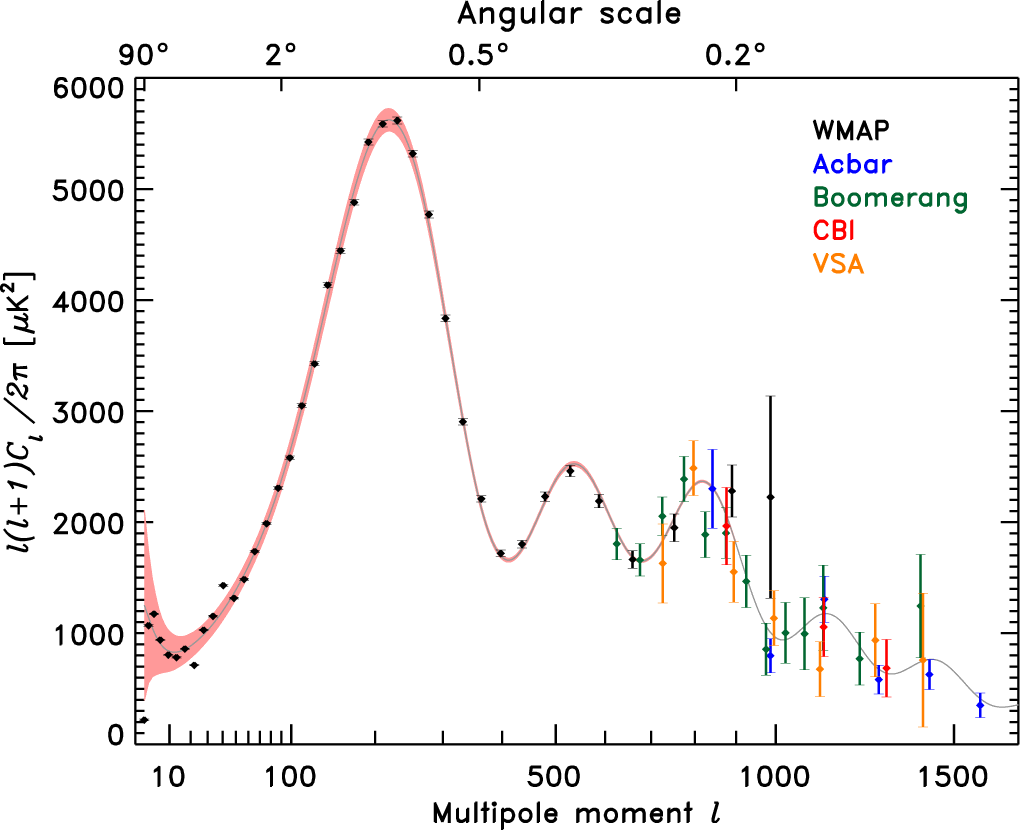
\includegraphics[width=0.8\textwidth]{cmb_spectrum_ped.png}
        \caption{Figure showing the power spectrum from \cite{cmb4ped}. Data
            from the Wilkinson Microwave Anisotropy Probe (WMAP) with high-$l$
            values coming from various other collaborations shown in diagram.,
            figure originally sourced from %\cite{wmap}
            . The plot is multipole
            moment against the historically utilized quantity TT
            (temperature-temperature correlation).}
    \end{figure}

    Given this explanation of the CMB in the CCM, we anticipate that the
    power spectrum will be dependent on the large scale structure formation of
    the cosmos, as we take the emitting and absorbing objects in $\bar{M}$ to
    be galaxies which have a known hierarchical structure. There are namely
    three large scale structures which we will concern ourselves with.
    \begin{itemize}
        \item Superclusters - a cluster of a cluster of galaxies
        \item Clusters  - a cluster of several galaxies 
        \item Galaxies - The galaxies themselves
    \end{itemize}
    Having only these structures, however, is perhaps not the most meaningful
    way to consider how the power spectrum will form. Along with these, there
    is a larger underlying structure, which has to do with the average void
    distance between these superclusters of galaxies. It is through these large
    structures and the numerical relationships between them, that the CCM must
    reproduce the power spectrum of the CMB.
    
    \subsubsection{Methodology}
    The principal concept of reproducing the power spectrum of the CMB in the
    CCM relies heavily on being able to reproduce the large scale structures
    mentioned above. Thus approaching this problem via simulation was a natural
    conclusion. The aim then will be to \textit{pack} super clusters of
    galaxies into an $\mathbb{S}^3$ surface area based on typical void size and
    number count. Doing so will rely on certain parameters which must be
    inputted manually and numerically (such as the radius of the $\mathbb{S}^3$
    universe, super cluster number count, void size, etc.) to then attempt to
    recover the power spectrum by projecting these objects onto the sky using
    some standard astrophysics libraries. 

    Exact numbers for galaxies per cluster and cluster per supercluster are few
    and far between, but approximations exist online which gave a reasonable
    starting estimate for the simulations. Exact parameters utilized will be
    discussed further in 3.2.4.
    
    \subsubsection{Simulations}
    The simulation itself is broken into two parts. The first part happens in
    Mathematica and is the more computationally expensive part. This consists
    of packing the $\mathbb{S}^3$ volume with the super clusters of galaxies.
    This is done by first selecting a number of super clusters (which in most
    cases we will consider to be on the order of $10^7$). From there, the super
    clusters are distributed throughout the $\mathbb{S}^3$ space according to a
    cubical packing\footnotemark (ie each void is modelled as a cube and 
    the super clusters are placed on each vertex of the vacuum cube). This
    is done uniformly and allows for one to discretize the volume of the
    universe into layers or shells, each of which containing a certain number
    of super clusters. After this packing is done, the super clusters are
    broken down into a specific number of clusters, and further into galaxies,
    thus adding many more points into the simulation (see Figure 3).

    \begin{figure}[h]
        \centering
        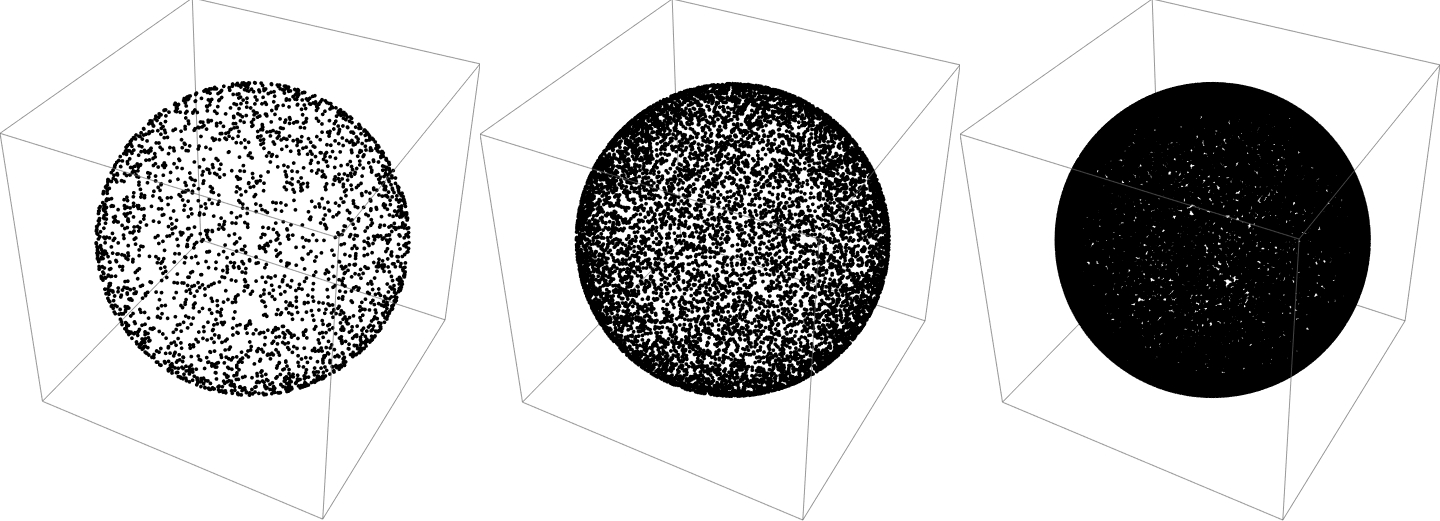
\includegraphics[width=0.8\textwidth]{Layers.jpg}
        \caption{Figures showing layer slicing of Mathematica simulation of
        cubical packing of super clusters. Left shows Layer 2, middle shows
        Layer 3, right shows Layer 10 of projected slices onto celestial sphere.}
    \end{figure}
    \begin{figure}[h]
        \centering
        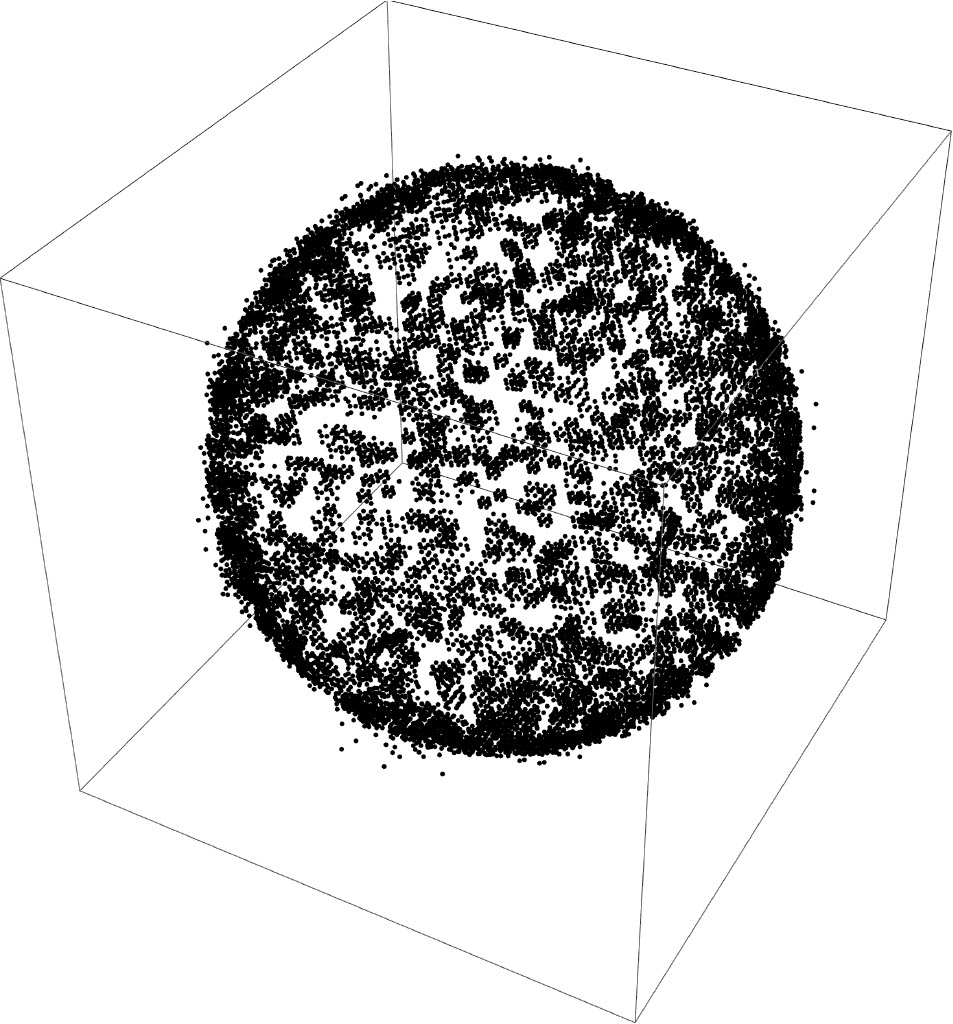
\includegraphics[width=0.6\textwidth]{layer_cluster.jpg}
        \caption{Replacement of super cluster points with clusters and galaxies
        for low $n$ layer.}
    \end{figure}

    \footnotetext{A cubical packing is at least a decent first guess. There are
    any number of different ways to pack the superclusters in any number of
    geometries, however for now only cubical packings will be considered. This will
    be discussed further in section 4}

    From here, the galaxies are projected onto celestial sphere layer by layer
    (a general depiction of this layering process can be seen in Figure 2).

    The output from this projection onto the celestial sphere is then fed into
    a python library called healpy which is a library built on HEALPix. The
    healpy library was developed to handle pixelated data on a sphere and
    HEALPix was developed precisely for efficient handling of data from the
    likes of WMAP and BOOMERANG. Thus, this software has plenty of tools for
    developing images of the sky and taking the pixelated data output from
    Mathematica and translating it into a power spectrum as well as a general
    temperature map of the sky.

    \subsubsection{Results}
    The results of running the simulation scheme mentioned above vary to some
    degree or another, largely depending on the ratio of the void size to the
    radius of the universe. However, certain sets of parameters produce power
    spectra that are of particular interest.

    First, it is worth using healpy on the WMAP data set in order to determine
    what the CMB power spectrum looks like using this software. Doing so
    results in Figure 4.

    \begin{figure}[h]
        \centering
        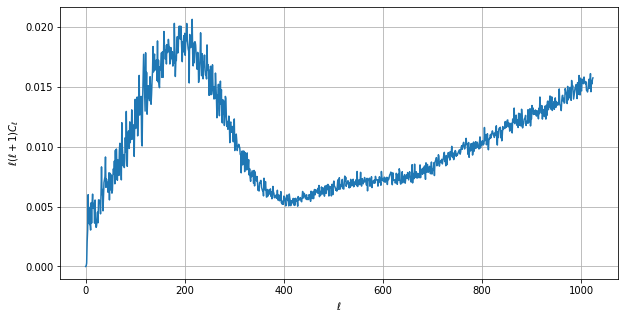
\includegraphics[width=\textwidth]{spectrum_real.png}
        \caption{The CMB power spectrum produced in healpy directly from the
            WMAP data. Notably, the Planck data is not used in this thesis as
            its resolution is quite high and comparing to a resolution that
            high would require significantly more computation time in the
            simulations where that resolution is generally not required for first
            order approximations.}
        %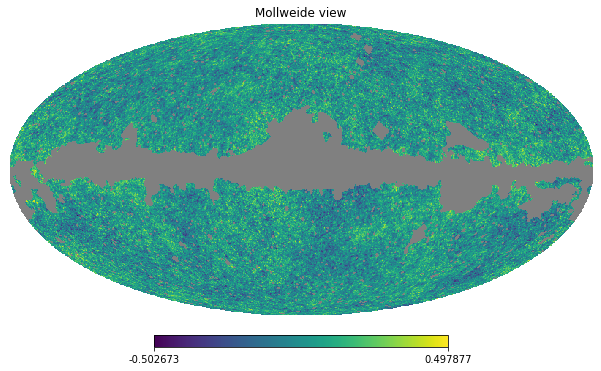
\includegraphics[width=0.7\textwidth]{mollweide_real.png}
    \end{figure}
    \begin{figure}[h!]
        \centering
        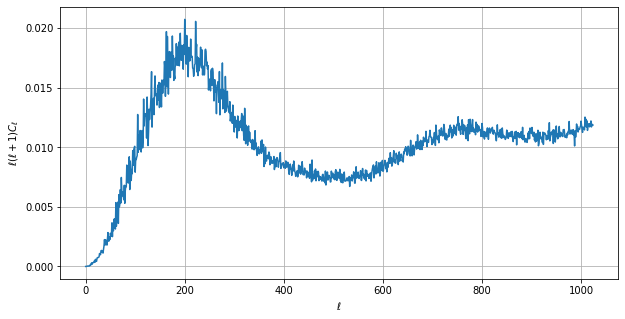
\includegraphics[width=\textwidth]{spectrum_ccm.png}
        \caption{The CMB power spectrum produced in healpy directly from the
            Mathematica output utilizing cubic packing. We note the
            spectrum is characteristically varied, and notably starts from
            zero, likely due to there being no constraint on how close exactly
            the packed superclusters are allowed to be to some origin point (the
            celestial sphere).}
        %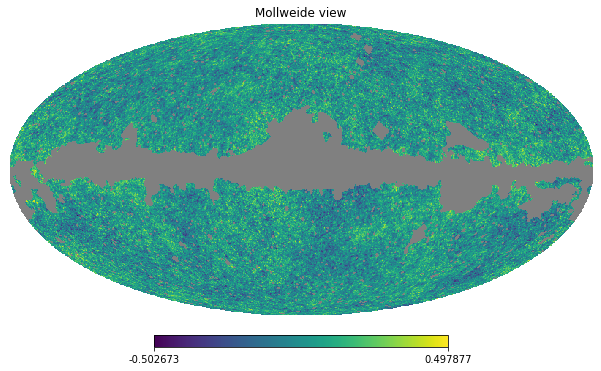
\includegraphics[width=0.7\textwidth]{mollweide_real.png}
    \end{figure}

    The results of running the simulation and developing the power spectrum
    from the output of the Mathematica code can be seen in Figure 5. This plot
    was simulated utilizing a supercluster count of $10^6$, with 9 clusters per
    supercluster, and 20 galaxies per cluster, totally out to 180 million
    galaxies in total. The void size if taken to be 10 Megaparsecs, which
    when utilizing a packing of this type, results in the radius of the
    $\mathbb{S}^3$ ball coming out to be 210 Megaparsecs.

    \subsubsection{Analysis}
    While a complete analysis of the average error between the two plots would
    certainly provide a rather complete and quantitative analysis of the Figures
    4 and 5, the results seem to be rather self explanatory in a more
    qualitative way. 

    The simulation utilizing cubical packing has reproduced to a reasonably
    high degree of accuracy the first major feature of the CMB. That being the
    first peak in the power spectrum at $l \approx 200$. Beyond the $l \approx
    400$ point, there are noticeable discrepancies, however the whole of this
    simulation is meant to provide merely a first (or more frankly a zeroth)
    order approximation to determine the feasibility of reproducing the CMB
    from first principles in the CCM. 

    An analysis comparing the two also does not entirely do justice to just how
    unique the result in Figure 5 is. It may seem as though, perhaps, any
    random scattering of the galaxies across the cosmos would likely produce a
    spectrum which may approximate a black body well enough construct this near
    black body spectrum. In order to show how this is not the case, we will do
    exactly this, and conduct the same analysis as done for Figure 5, however
    instead of cubically packing superclusters and then decomposing them into
    their constituent componenets thus creating large scale hierarchical
    structure, we will uniformly scatter 180 millions galaxies across the same
    cosmos. The result of this analysis is seen in Figure 6.

    \begin{figure}[h]
        \centering
        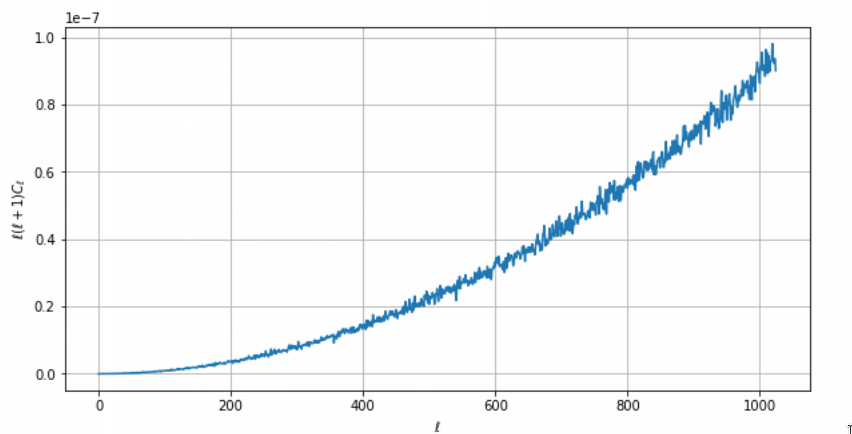
\includegraphics[width=\textwidth]{spectrum_rand_full.png}
        \caption{The CMB power spectrum produced in healpy directly from the
            Mathematica output utilizing completely random packing. We note
            that there is no apparent structure to the spectrum, and also that
            the scale of the vertical axis has changed
            considerably}
    \end{figure}

    Notably, the spectrum from the completely random scattering has no
    structure even remotely similar to a typical black body spectrum nor the
    CMB power spectrum. This highlights the fact that there is something unique
    about the packing of the clusters of galaxies in the cosmos and the
    detected power spectrum within the CCM. Further, the deviations noted
    between the simulated power spectrum and the true power spectrum past the $l
    \approx 400$ point could possibly be resolved by an alternate packing
    geometry, or various ratios of void size to cosmic radius. 

    As stated previously however, replicating the exact power spectrum is
    outside the bounds of this thesis. Doing so is likely an exercise in
    searching a wide parameter space for possible values which could reproduce
    various characteristics of the known power spectrum. However, it would
    appear that the CCM can, at the very least, reproduce the primary
    characteristics of the CMB, which is certainly a surprising result to fall
    out of such an approximate analysis.
    \newpage
    \section{Further Research}
    \subsection{CMB Temperature}
    The calculation conducted throughout 3.1 provided a general overview of how
    the CMB functions within the chronometric model, and while the result of
    $T\approx 2.54$ K is promising in the context of reproducing the CMB in this
    model, it is not as complete an analysis as might be hoped.
    
    There is the question of what exactly the "average" galaxy is in the
    context of the calculations in 3.1. The utilization of the Milky Way may or
    may not be entirely accurate, and, for instance, if one conducts the same
    analysis as found in 3.1.5, they will find the Andromeda galaxy (Messier
    31) yields an average temperature of $\sim 3.17$ K. For general purposes we
    assumed the luminosities of the galaxies to be approximately equal, thus
    implying that there may be some mean distribution from which one can
    draw an average luminosity value. However, discerning these figures is not
    quite as straight forward. Astronomical measurements are subject to
    uncertainties coming from various sources, and in particular magnitude
    suffers from this. Thus, figures for these values vary largely between
    sources depending on the equipment and methods utilized. Further research
    is required for determining selection of this data so that a better
    understanding of the average temperature can be formed.
    \subsection{CMB Power Spectrum}
    The power spectrum simulation, while reproducing the primary 
    characteristics of the experimentally observed power spectrum, is not
    exactly in line with the expected. While it would be perhaps foolish to
    assume that such an approximate simulation of the cosmos could produce an
    exact replica of the data, it would be ideal if the discrepancies following
    the $l=400$ multipole moment could be brought into a smaller range. How
    exactly to do this, though, is a topic in searching a wide space of
    parameters in which there is not much direction to work from.

    \subsection{The Redshift}
    As stated in section 1.1, an analysis of the number count to redshift
    relation and magnitude to redshift relation has already been
    conducted to reasonable depth by Kaye in \cite{kaye} utilizing modern
    astrophysical data. However, in light of new, high redshift data coming in
    from JWST as mentioned in \cite{labbe}, there will be a much larger pool of
    data to operate with than in the past, and at $z$ values never before
    observed.
    \newpage

    \section{Conclusion}
    Throughout the course of this thesis we have explored a truly fantastical
    cosmological model. It is a world vastly unfamiliar to our intuitions as
    physicists and perhaps that is what drives its appeal. However, the
    question of whether this model is a mere toy in the sandbox of mathematics or a
    possible description of the universe we inhabit is yet unanswered. 

    While the world described in the Chronometric Model may feel overly
    simplisitc, appealing to the early Einstein universe as a static 3-sphere
    with no concept or care for a beginning or end, it is perhaps precisely in
    this simplicity which we find its appeal. The Standard Cosmological model
    calls for dark matter and dark energy, a period of exponential inflation,
    and several free parameters in order to describe the cosmos at large,
    whereas the Chronometric Cosmos could not be more simple in its
    formulation and description of the observed universe. This disregard for
    the many parameters and place holders established by the Standard Model,
    along with a more rigorous mathematical underlying structure, only add to
    the model's inherit beauty. This is perhaps no more true than now, in a
    time where the Hubble parameter measurements are no longer overlapping in
    error, and as the fundamental concepts of early galaxy formation are
    beginning to come under question \cite{labbe} \cite{hub_const}.

    While the beauty of the model is certainly notable, it remains critical to
    consider it from the perspective of what is and isn't physically possible.
    In Kaye \cite{kaye} an analysis of the cosmological redshift ($z$-$N(z)$
    and $z$-$M(z)$) was conducted in which the Chronometric Redshift relation
    was put to the test of modern data. Reasonable (and sometimes perhaps even
    great) agreement was shown between CCM predictions and data, thus showing
    that the Chronometric Model is not falsified by the redshift measurements
    at hand. In this thesis, the Chronometric Model was put to the test of
    reproducing yet another critical phenomena in modern cosmology; the CMB. It
    was shown that the two major characteristics of the CMB are in fact able to
    be reproduced in a first order approximation thus further solidifying
    Segal's theory as not yet falsified in light of modern data.

    In physics, it is our job to probe the very nature of the universe, and in
    doing so gain some understanding of our surroundings much larger than
    ourselves. While the efficacy of Segal's theory as an overall description
    of the universe remains to be seen, there is certainly no doubt in its
    ability to reproduce critical aspects of modern cosmological data from
    first order approximations, which is why the Chronometric model has been and
    continues to be an important line of consideration.
    \section{Acknowledgments}
    First and foremost I would like to acknowledge Krzysztof Sliwa for his
    continued guidance, patience, and mentorship, and to thank him for sharing
    this wonderful research experience with me.

    I'd also like to thank Maxwell Kaye for sharing his experience in this
    research with me early on.

    Lastly I'd like to thank Debbie and Andy Burwig as well as Teo Patrosio and
    my wonderful housemates and friends for supporting me throughout all my
    endeavors, even if I wasn't always the most well prepared for them.
    \newpage
    \setstretch{1.0}

    \bibliographystyle{plain} % We choose the "plain" reference style
    \nocite{*}
    \bibliography{myref.bib} % Entries are in the refs.bib file




\end{document}
